\chapter{Moduly}

\section{Přidávání nových modulů}
Nové moduly se nahrávají do složky \textit{modules},
která leží vedle adresářů \textit{frontend}, \textit{backend} a \textit{uploads}.
Nahrávat lze jednotlivé html soubory, složky se složitější architekturou nebo
celé npm balíčky s vlastní zkompilovanou stránkou. Moduly by měly být nezávislé na
obsahu diskového prostoru v \uv{rodiči} a měly by tedy být samostatně spustitelné,
maximálně s interakcí s API.

\section{Aktuálně nasazené moduly}

\subsection{Modul hologram}
Tento modul bude sloužit na výstavě Pramenů Krkonoš k zobrazování 3D objektů ve formě hologramu,
který se bude pomalu otáčet a ukáže se tak návštěvníkovi ze všech stran.

\subsubsection{Načítání modulu}
Tento modul obsahuje velkou knihovnu, a tudíž není efektivní jej mít v primární aplikaci.
Protože by se tyto knihovny načítaly, i když by uživatel s tímto modulem neměl v plánu pracovat.
Což většinu času nebude chtít, a tudíž by to pouze vedlo ke zpomalení systému.
Systémem \textit{Lazy} načítání je tedy celý modul odříznut a načítá se až explicitně při jeho použití.

\subsubsection{Grafický engine}
Pro vykreslování 3D modelu na webu slouží WebGL, grafická knihovna podobná staré verzi OpenGL.
Reálně jsou dostupné dvě propracované knihovny pro práci ve WebGL.
ThreeJS, které se zaměřuje na statické vykreslování a předvádění.
BabylonJS, která naopak napodobuje známé programy jako je \textit{unity} a má podporu
fyziky a dalších podknihoven užitečných pro tvorbu her.
Pokud pomineme možnost naprogramovat vše od základu, nejvhodnější knihovnou 
je \textbf{ThreeJS}.\\
Z této knihovny využijeme moduly pro načítání modelu a textury, jejich spárování a
efektu Peppers Ghost, který je implementován pomocí 4 nezávislých kamer.


\subsubsection{Peppers Ghost Effect}
\begin{figure}[H]
	\centering
	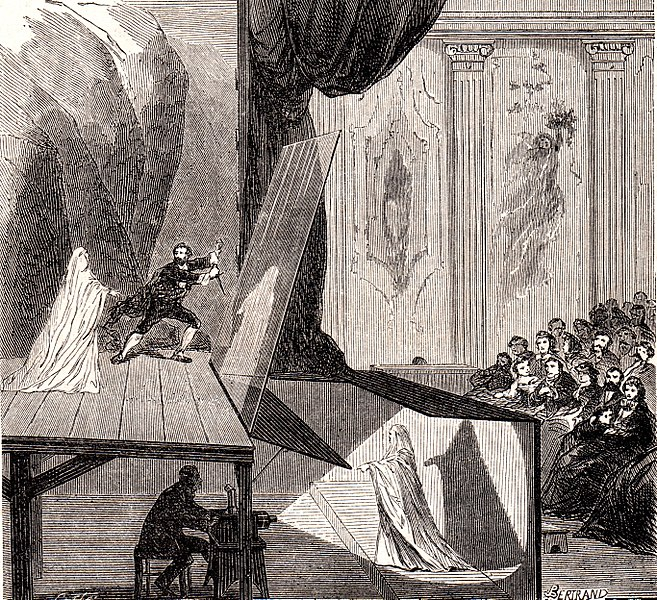
\includegraphics[width=.5\textwidth]{img/Peppers_Ghost.jpg}
	\caption[Peppers Ghost efekt - zdroj: \url{https://commons.wikimedia.org/wiki/File:Peppers_Ghost.jpg}]{Peppers Ghost efekt}
\end{figure}

Jedná se o divadelní trik, jež skládá pozorovateli dva obrazy přes sebe a vytváří iluzi
hologramu nebo ducha. Původně byl vyvinut pro divadelní představení, v moderní
době však dokáže simulovat i hologram, který známe ze sci-fi.

\subsubsection{Modely a textury}
Modely jsou z webu \url{https://3dwarehouse.sketchup.com} a
textury z webu \url{https://www.textures.com/ a https://texturehaven.com/}.\\
V programu blender pak byly tyto textury namapovány na objekt a bylo do nich
zapečeno ambient oclusion (stíny vytvořené stísněným prostorem).



\subsection{Prohlížeč map}
Dalším historickým prvkem, který bychom návštěvníkům této aplikace poskytli, jsou
2D mapy z 19. století. Uživatel si může vybrat mapu a tu si velmi podrobně
prohlížet pomocí přibližování a posouvání.

\subsubsection{Zdroj map}
Mapy byly získány od ČUZK výměnou za jejich kompletaci.
Mapu jsme totiž dostali ve formě \uv{tady máš puzzle a poslepujte si to sami}.
Každou mapu jsme tedy pečlivě zrekonstruovali, při zachování všech detailů a
historických přesností a bez jejich upravování či umělého přidávání.
